\documentclass[]{article}

\usepackage{graphicx,type1cm,eso-pic,color}
\usepackage[spanish]{babel} %%%% for


\makeatletter
          \AddToShipoutPicture{
            \setlength{\@tempdimb}{.95\paperwidth}
            \setlength{\@tempdimc}{.5\paperheight}
            \setlength{\unitlength}{1pt}
            \put(\strip@pt\@tempdimb,\strip@pt\@tempdimc){
        \makebox(0,0){\rotatebox{-90}{\textcolor[gray]{0.90}
        {\fontsize{.65cm}{.5cm}\selectfont{\rm Dae-Jin Lee}}}}
            }
        }
          \AddToShipoutPicture{
            \setlength{\@tempdimb}{.50\paperwidth}
            \setlength{\@tempdimc}{.95\paperheight}
            \setlength{\unitlength}{1pt}
            \put(\strip@pt\@tempdimb,\strip@pt\@tempdimc){
        \makebox(0,0){\rotatebox{0}{\textcolor[gray]{0.90}
        {\fontsize{.5cm}{.5cm}\selectfont{\rm Curso de Estad\'istica b\'asica para Data Scientist  - @datahack}}}}
            }
        }
\makeatother

\def\tightlist{}

\usepackage{lmodern}
\usepackage{amssymb,amsmath}
\usepackage{ifxetex,ifluatex}
\usepackage{fixltx2e} % provides \textsubscript
\ifnum 0\ifxetex 1\fi\ifluatex 1\fi=0 % if pdftex
  \usepackage[T1]{fontenc}
  \usepackage[utf8]{inputenc}
\else % if luatex or xelatex
  \ifxetex
    \usepackage{mathspec}
    \usepackage{xltxtra,xunicode}
  \else
    \usepackage{fontspec}
  \fi
  \defaultfontfeatures{Mapping=tex-text,Scale=MatchLowercase}
  \newcommand{\euro}{???}
\fi
% use upquote if available, for straight quotes in verbatim environments
\IfFileExists{upquote.sty}{\usepackage{upquote}}{}
% use microtype if available
\IfFileExists{microtype.sty}{%
\usepackage{microtype}
\UseMicrotypeSet[protrusion]{basicmath} % disable protrusion for tt fonts
}{}
\usepackage{graphicx}
\makeatletter
\def\maxwidth{\ifdim\Gin@nat@width>\linewidth\linewidth\else\Gin@nat@width\fi}
\def\maxheight{\ifdim\Gin@nat@height>\textheight\textheight\else\Gin@nat@height\fi}
\makeatother
% Scale images if necessary, so that they will not overflow the page
% margins by default, and it is still possible to overwrite the defaults
% using explicit options in \includegraphics[width, height, ...]{}
\setkeys{Gin}{width=\maxwidth,height=\maxheight,keepaspectratio}
\ifxetex
  \usepackage[setpagesize=false, % page size defined by xetex
              unicode=false, % unicode breaks when used with xetex
              xetex]{hyperref}
\else
  \usepackage[unicode=true]{hyperref}
\fi
\hypersetup{breaklinks=true,
            bookmarks=true,
            pdfauthor={Dae-Jin Lee \textless{} lee.daejin@gmail.com \textgreater{}},
            pdftitle={Curso de Estadística básica para Data Scientists},
            colorlinks=true,
            citecolor=blue,
            urlcolor=blue,
            linkcolor=magenta,
            pdfborder={0 0 0}}
\urlstyle{same}  % don't use monospace font for urls
\setlength{\parindent}{0pt}
\setlength{\parskip}{6pt plus 2pt minus 1pt}
\setlength{\emergencystretch}{3em}  % prevent overfull lines
\setcounter{secnumdepth}{5}

\title{\textbf{Curso de Estadística básica para Data Scientists}}
\author{Dae-Jin Lee \textless{}
\href{mailto:lee.daejin@gmail.com}{\nolinkurl{lee.daejin@gmail.com}}
\textgreater{}}
\date{\textbf{TEMA 3. Estadística descriptiva bivariante}}

\usepackage{amsfonts}
\usepackage{amsmath}
\usepackage{amssymb}
\usepackage{natbib}
%\usepackage[T1]{fontenc}
\usepackage{latexsym}
\usepackage{graphicx}
\usepackage{caption}
\usepackage{subcaption}
\usepackage{color}
\usepackage{algorithm2e}
%%
%     Definitions
%
\newcommand{\tri}{\bigtriangleup}
\newcommand{\Xp}{X^\prime}
\newcommand{\E}{\mbox{E}}
\newcommand{\Hh}{\mbox{H}}
\newcommand{\V}{\mbox{Var}}
\newcommand{\tr}{\mbox{tr}}
\newcommand{\CV}{\mbox{CV}}
\newcommand{\GCV}{\mbox{GCV}}
\newcommand{\AIC}{\mbox{AIC}}
\newcommand{\ph}{\phantom{0}}
\newcommand{\half}{\mbox{${1\over2}$}}
\newcommand{\bfzero}{\boldsymbol{0}}
\newcommand{\bfone}{\boldsymbol{1}}

\newcommand{\bfa}{\boldsymbol{a}}
\newcommand{\bfb}{\boldsymbol{b}}
\newcommand{\bfe}{\boldsymbol{e}}
\newcommand{\bff}{\boldsymbol{f}}
\newcommand{\bfg}{\boldsymbol{g}}
\newcommand{\bfs}{\boldsymbol{s}}
\newcommand{\bfu}{\boldsymbol{u}}
\newcommand{\bfx}{\boldsymbol{x}}
\newcommand{\bfy}{\boldsymbol{y}}
\newcommand{\bfz}{\boldsymbol{z}}

\newcommand{\bfA}{\boldsymbol{A}}
\newcommand{\bfB}{\boldsymbol{B}}
\newcommand{\bfC}{\boldsymbol{C}}
\newcommand{\bfD}{\boldsymbol{D}}
\newcommand{\bfF}{\boldsymbol{F}}
\newcommand{\bfG}{\boldsymbol{G}}
\newcommand{\bfH}{\boldsymbol{H}}
\newcommand{\bfI}{\boldsymbol{I}}
\newcommand{\bfM}{\boldsymbol{M}}
\newcommand{\bfP}{\boldsymbol{P}}
\newcommand{\bfQ}{\boldsymbol{Q}}
\newcommand{\bfR}{\boldsymbol{R}}
\newcommand{\bfS}{\boldsymbol{S}}
\newcommand{\bfT}{\boldsymbol{T}}
\newcommand{\bfU}{\boldsymbol{U}}
\newcommand{\bfV}{\boldsymbol{V}}
\newcommand{\bfW}{\boldsymbol{W}}
\newcommand{\bfX}{\boldsymbol{X}}
\newcommand{\bfY}{\boldsymbol{Y}}
\newcommand{\bfZ}{\boldsymbol{Z}}


\newcommand{\bfalpha}{\boldsymbol{\alpha}}
\newcommand{\bfbeta}{\boldsymbol{\beta}}
\newcommand{\bfepsilon}{\boldsymbol{\epsilon}}
\newcommand{\bfgamma}{\boldsymbol{\gamma}}
\newcommand{\bfGamma}{\boldsymbol{\Gamma}}
\newcommand{\bfmu}{\boldsymbol{\mu}}
\newcommand{\bfeta}{\boldsymbol{\eta}}
\newcommand{\bfrho}{\boldsymbol{\rho}}
\newcommand{\bftheta}{\boldsymbol{\theta}}
\newcommand{\bfxi}{\boldsymbol{\xi}}
\newcommand{\bftau}{\boldsymbol{\tau}}
\newcommand{\bflambda}{\boldsymbol{\lambda}}
\newcommand{\bfsigma}{\boldsymbol{\sigma}}
\newcommand{\bfLambda}{\boldsymbol{\Lambda}}
\newcommand{\bfSigma}{\boldsymbol{\Sigma}}

\renewcommand{\theequation}{\thesection.\arabic{equation}}
\numberwithin{equation}{section}

\begin{document}
\maketitle

{
\hypersetup{linkcolor=black}
\setcounter{tocdepth}{2}
\tableofcontents
}
\newpage

\href{https://idaejin.github.io/bcam-courses/R/datahack/}{Regresar a la
página principal}

\section{Estadística descriptiva
bivariante}\label{estadistica-descriptiva-bivariante}

En el tema anterior hemos visto cómo describir una muestra de datos de
una variable mediante:

\begin{itemize}
\tightlist
\item
  Representaciones gráficas
\item
  Estadísticos (de posición, dispersión, etc \ldots{})
\end{itemize}

En este tema consideraremos el caso de 2 variables. Nuestro interés será
por tanto, saber si \(Y\) es otra variable definida sobre la misma
población que \(X\), ¿será posible determinar si existe alguna relación
entre \(X\) e \(Y\)?

Ahora tomamos dos medidas a cada individuo de la muestra. Consideramos
una población de \(n\) individuos, donde cada uno de ellos presenta dos
características que representamos mediante las variables \(X\) e \(Y\).

Las variables pueden ser cuantitativas, discretas o continuas o
cualitativas, dando lugar a muchas combinaciones:

\begin{itemize}
\tightlist
\item
  cualitativa/cualitativa, discreta/continua, continua/continua, etc.
\end{itemize}

El tipo de análisis dependerá de la combinación que tengamos.

Tomamos una muestra de la población y medimos las variables (\(X\) e
\(Y\)), esa muestra estará dividida en clases para cada una de las
variables y existirán elementos que pertenezcan a las distintas
combinaciones de las clases.

\subsection{Distribuciones de
frecuencias}\label{distribuciones-de-frecuencias}

Llamamos \textbf{distribución conjunta de frecuencias} de dos variables
(\(X\) e \(Y\)) a la tabla que representa los valores observados y las
frecuencias relativas/absolutas de cada par.

\subsubsection{Distribución conjunta}\label{distribucion-conjunta}

Consideramos una población de \(n\) individuos, donde cada uno de ellos
presenta dos caracteres que representamos mediante las variables \(X\) e
\(Y\). Representamos mediante:+

\[
X \rightarrow x_1,x_2,...,x_k
\] las \(k\) modalidades que presenta la variable \(X\) y mediante \[
Y \rightarrow y_1,y_2,...,y_p
\] las \(p\) modalidades de \(Y\).

Con la intención de reunir en una sola estructura toda la información
disponible, creamos una tabla formada por \(k\times p\) casillas,
organizadas de forma que se tengan \(k\) filas y \(p\) columnas. La
casilla denotada de forma general mediante el subíndice \(_{ij}\) hará
referencia a los elementos de la muestra que presentan simultáneamente
las modalidades \(x_i\) e \(y_j\).

\includegraphics[width=0.65000\textwidth]{pics/frectab2abs.png}

De este modo, para \(i=1,...,k\),y para \(j=1,...,p\),se tiene que
\(n_{ij}\) \(ij\) es el número de individuos o frecuencia absoluta, que
presentan a la vez las modalidades \(x_i\) e \(y_j\).

El número de individuos que presentan la modalidad \(x_i\), es lo que
llamamos frecuencia absoluta marginal de \(x_i\) y se representa como
\(n_{i\cdot}\), donde

\[
    n_{i\cdot} = n_{i1}+n_{i2} + ... + n_{ip} = \sum_{j=1}^{p} n_{ij}
\]

El símbolo \(\cdot\) en \(n_{i\cdot}\) simboliza que estamos
considerando los elementos de \(x_i\) independientemente de los valores
de \(Y\). De forma análoga, se define la frecuencia absoluta marginal de
la modalidad \(y_j\) como: \[
    n_{\cdot j} = n_{1j}+n_{2j} + ... + n_{kj} = \sum_{i=1}^{k} n_{ij}
\]

\textbf{Propiedad}

\[
    n_{\cdot\cdot} = \sum_{i=1}^{k}\sum_{j=1}^{p} n_{ij}  = n
\]

\subsubsection{Distibución marginal}\label{distibucion-marginal}

A la proporción de elementos (tanto por uno) que presentan
simultáneamente las modalidades \(x_i\) e \(y_j\) la llamamos frecuencia
relativa \(f_{ij}\)

\[
    f_{ij} = \frac{n_{ij}}{n}
\] siendo las frecuencias relativas marginales:

\[
      f_{i\cdot} = \sum_{j=1}^{p}f_{ij}\frac{n_{i\cdot}}{n}
\] \[
      f_{\cdot j} = \sum_{i=1}^{k}f_{ij}\frac{n_{\cdot j}}{n}
\]

\includegraphics[width=0.65000\textwidth]{pics/frectab2rel.png\#center}

\textbf{Propiedad}

\[
    f_{\cdot\cdot} = \sum_{i=1}^{k}\sum_{j=1}^{p} f_{ij} = 1
\]

\subsubsection{Distribución
condicionada}\label{distribucion-condicionada}

De todos los elementos de la población, \(n\), podemos estar
interesados, en un momento dado, en un conjunto más pequeño que está
formado por aquellos elementos que han presentado la modalidad
\(y_j\),par aalgún \(j=1,...,p\) .El número de elementos de este
conjunto sabemos que es \(n_{\cdot j}\). La variable \(X\) definida
sobre este conjunto se denomina variable condicionada y se suele denotar
mediante \(X|y_j\) o bien \(X|Y=y_j\).

La distribución de frecuencias absolutas de esta nueva variable es
exactamente la columna \(j\) de la tabla. Por tanto sus frecuencias
relativas, que denominaremos frecuencias relativas condicionadas son

\[
    f_j^{i} = \frac{n_{ij}}{n_{\cdot j}} \mbox{ para todo $i= 1,...,k$}
\]

Del mismo modo, la variable condicionada \(Y|x_i\) cuya distribución de
frecuencias relativas condicionadas es: \[
    f_i^{j} = \frac{n_{ij}}{n_{i\cdot}} \mbox{ para todo $j= 1,...,p$}
\]

\subsection{Representaciones gráficas}\label{representaciones-graficas}

Dependerá del tipo de variables con las que estemos trabajando y de si
están agrupadas o no.

\begin{itemize}
\tightlist
\item
  Cualitativas , Cuantitativas discretas:
\item
  Cuantitativas continuas:
\end{itemize}

\subsubsection{Diagramas de barras en 3 dimensiones para datos
agrupados}\label{diagramas-de-barras-en-3-dimensiones-para-datos-agrupados}

\textbf{Ejemplo (continua/continua), en datos agrupados:} A continuación
se muestran los datos recogidos de medir la longitud (X en mm) y el peso
(Y en gr) de una muestra de 117 tornillos producidos por una máquina.

\includegraphics[width=0.85000\textwidth]{pics/tab2x2.png\#center}

\begin{figure}

{\centering 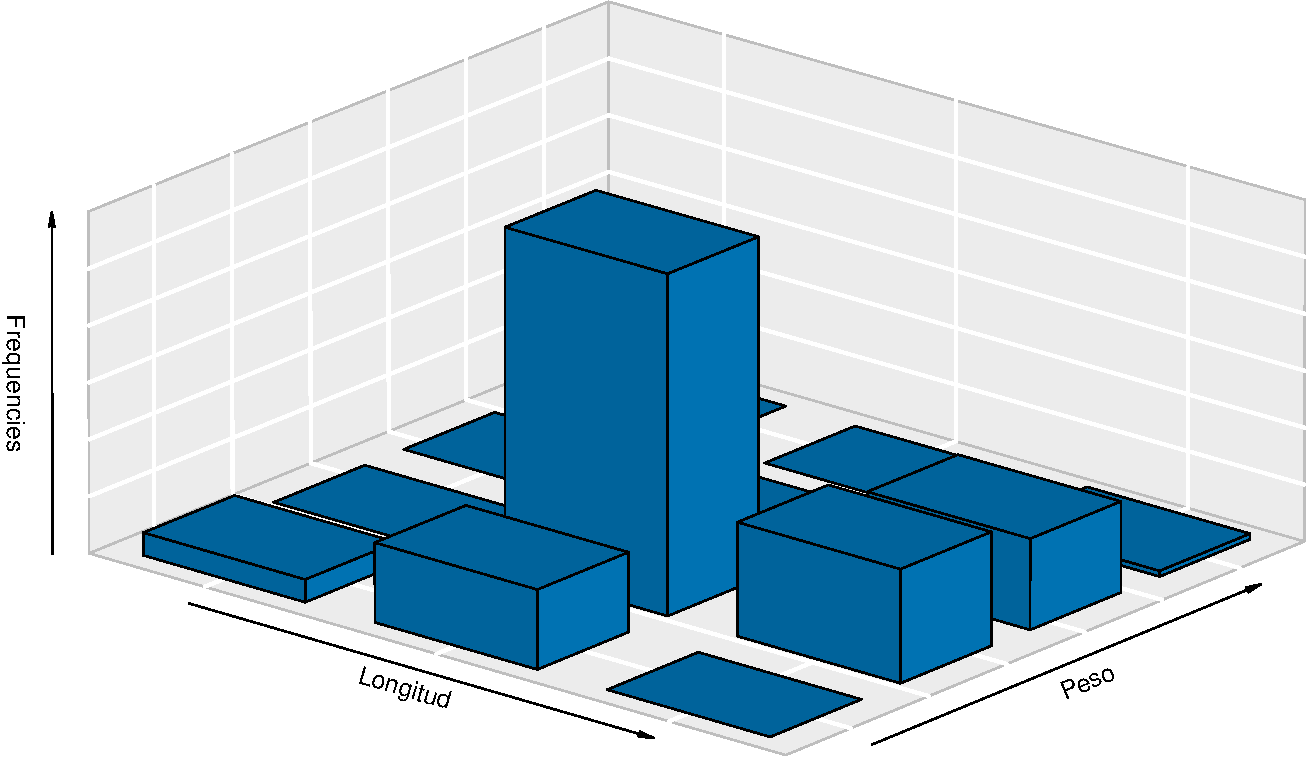
\includegraphics{tema3_files/figure-latex/unnamed-chunk-1-1} 

}

\caption{Histograma en 3 dimensiones}\label{fig:unnamed-chunk-1}
\end{figure}

\subsubsection{Diagrama de dispersión}\label{diagrama-de-dispersion}

La representación gráfica más útil para mostrar el tipo de relación
entre dos variables continuas sin agrupar es el diagrama de dispersión,
que representa cada par de puntos \((x_i,y_i)\), \(i=1,...n\), en un
plano cartesiano.

Supongamos que tenemos las 117 mediciones de los tornillos sin agrupar.
La siguiente figura muestra un gráfico de dispersión, que nos permite
intuir la relación entre el Peso y la Longitud.

\begin{figure}

{\centering 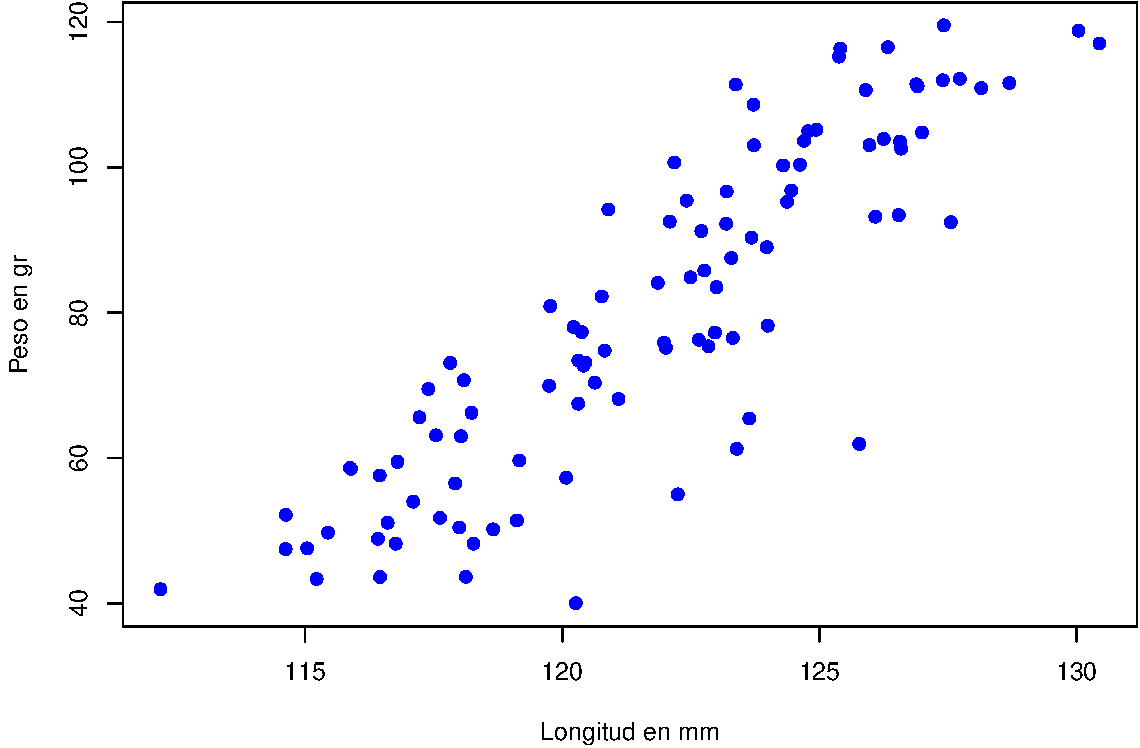
\includegraphics{tema3_files/figure-latex/unnamed-chunk-2-1} 

}

\caption{Gráfico de dispersión Longitud/Peso}\label{fig:unnamed-chunk-2}
\end{figure}

\begin{figure}

{\centering 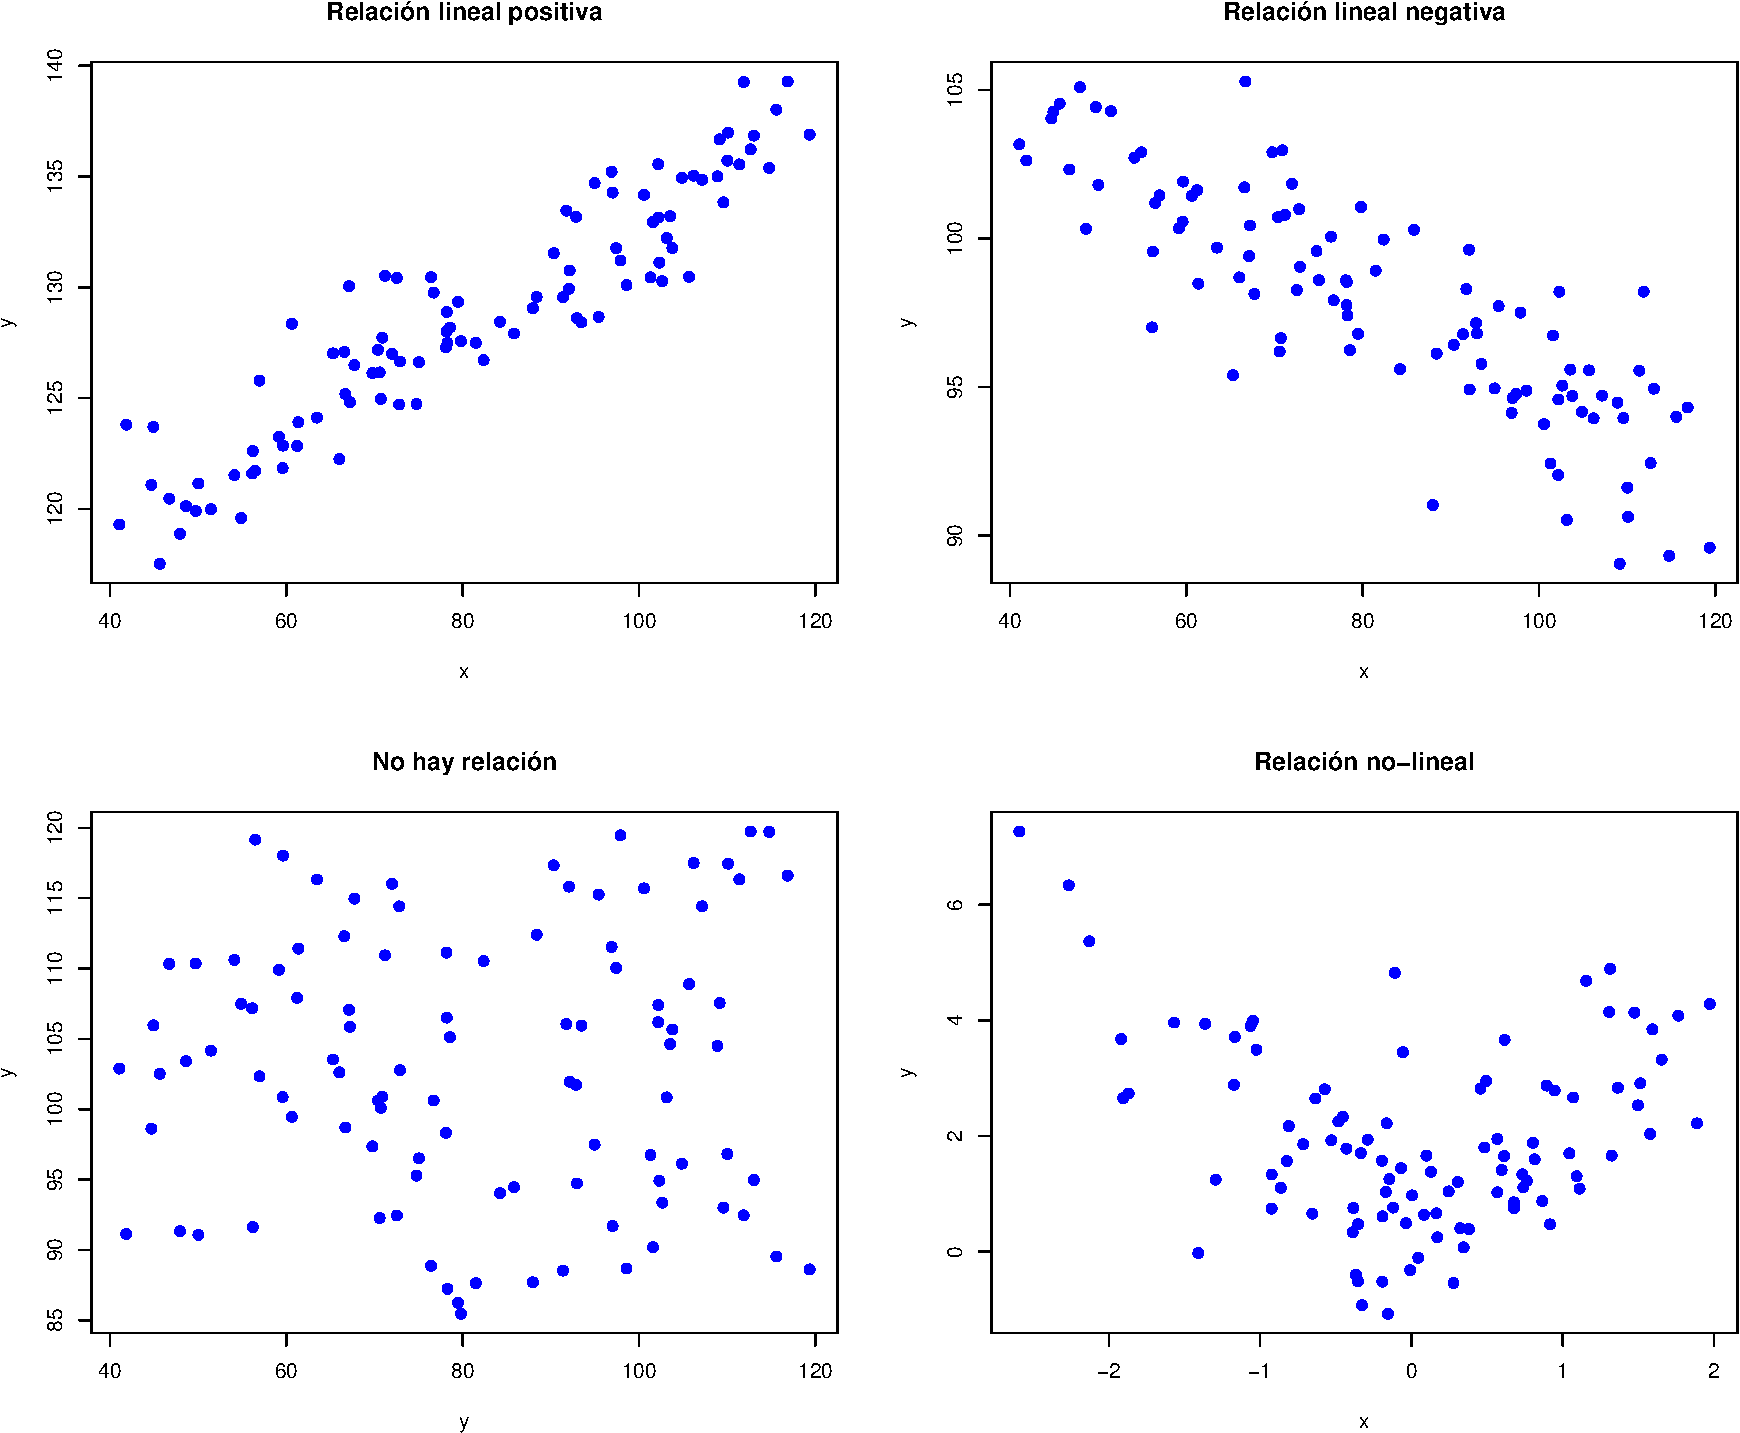
\includegraphics{tema3_files/figure-latex/unnamed-chunk-3-1} 

}

\caption{Tipos de relaciones X/Y en diagramas de dispersión}\label{fig:unnamed-chunk-3}
\end{figure}

\subsection{Medidas de dependencia
lineal}\label{medidas-de-dependencia-lineal}

Las dos medidas más utilizadas para cuantificar el grado y el sentido de
la dependencia lineal son: la covarianza y la correlación.

\subsubsection{Covarianza}\label{covarianza}

Nos indica si la relación entre las variables es positiva o negativa Su
magnitud depende de las unidades

Cuando los datos están agrupados en forma de tabla:

\[
    S_{xy} = \sum_i \sum_j f_{ij}(x_i-\bar{x})(y_i-\bar{y}) = \sum_i \sum_j f_{ij}x_i y_j - \bar{x}\bar{y}
\]

\emph{Ejercicio:} Supongamos la siguiente tabla donde
\texttt{X=Nº\ de\ hermanos} e \texttt{Y=Nº\ de\ suspensos}

\url{https://www.youtube.com/watch?v=zWXwwFJwCZE}

\includegraphics[width=0.42500\textwidth]{pics/XY1.png\#center}

Cálculo de marginales

\includegraphics[width=0.45000\textwidth]{pics/XY2.png\#center}

Cálculo de medias marginales

\includegraphics[width=0.75000\textwidth]{pics/XY3.png\#center}

\[
\begin{aligned}
      S_{xy} = \frac{\sum f_{ij}x_i y_j}{n} - \bar{x}\bar{y} & = \frac{0\cdot 0 \cdot 4 + 0\cdot 0 \cdot 5 + 0\cdot 2 \cdot 2 + 0\cdot 3  + ... + 3\cdot 3 \cdot 1}{50} - 1.48\times 1.32 = \\
             & = \frac{104}{50} - 1.9536 = 0.1264
\end{aligned}
\]

\includegraphics[width=0.55000\textwidth]{pics/XY4.png\#center}

\includegraphics[width=0.55000\textwidth]{pics/XY5.png\#center}

\end{document}